\chapter{Miscellaneous Algorithms}

\section{IOU (Intersection over Union) \cite{medium/analytics-vidhya/iou-intersection-over-union-705a39e7acef}}\label{IOU (Intersection over Union)}

\begin{table}[H]
    \begin{minipage}[b]{0.325\linewidth}
        \begin{figure}[H]
            \centering
            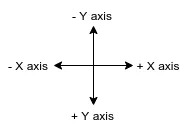
\includegraphics[width=\linewidth, height=6cm, keepaspectratio]{Pictures/ds-algo/iou-cs.jpg}
            \caption{IOU: Co-ord. System}
        \end{figure}
    \end{minipage}
    \hfill
    \begin{minipage}[b]{0.325\linewidth}
        \begin{figure}[H]
            \centering
            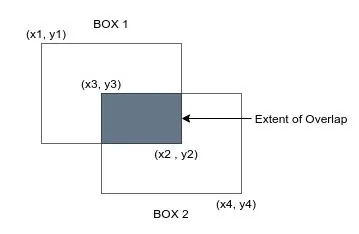
\includegraphics[width=\linewidth, height=6cm, keepaspectratio]{Pictures/ds-algo/iou-1.jpg}
            \caption{IOU: Input/ Scenario}
        \end{figure}
    \end{minipage}
    \hfill
    \begin{minipage}[b]{0.325\linewidth}
        \begin{figure}[H]
            \centering
            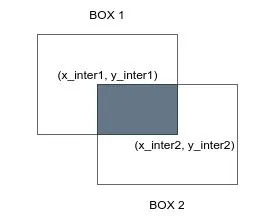
\includegraphics[width=\linewidth, height=6cm, keepaspectratio]{Pictures/ds-algo/iou-4.jpg}
            \caption{IOU: Intersection}
        \end{figure}
    \end{minipage}
\end{table}

\[
    \hfill
    \displaystyle IOU = \dfrac{\text{Area of Intersection of 2 boxes}}{\text{Area of Union of 2 boxes}}
    \hfill
\]

\begin{adjustwidth}{-2cm}{-2cm}

\[
    x_{inter1} = \max(x_1, x_3) 
    \hfill 
    y_{inter1} = \max(y1, y_3)
    \hfill
    x_{inter2} = \max(x_2, x_4) 
    \hfill 
    y_{inter2} = \max(y_2, y_4)
    \hfill
\]
\[
    width_{inter} = (x_{inter2} - x_{inter1})
    \hfill
    height_{inter} = (y_{inter2} - y_{inter1})
    \hfill
\]
\[
    area_{inter} = width_{inter} * height_{inter}
    \hfill
\]
\[
    area_{box1} = (x_2 - x_1) * (y_2 - y_1)
    \hfill
    area_{box2} = (x_4 - x_2) * (y_4 - y_2)
    \hfill
\]
\[
    area_{union} = area_{box1} + area_{box2} - area_{inter}
    \hfill
\]
\[
    IOU = \dfrac{area_{inter}}{area_{union}} \in [0,1]
    \hfill
\]

\end{adjustwidth}

\begin{enumerate}
    \item IOU(Intersection over Union) is a term used to describe the extent of overlap of two boxes. 
    
    \item The greater the region of overlap, the greater the IOU.

    \item IOU is mainly used in applications related to object detection, where we train a model to output a box that fits perfectly around an object.

    \item IOU is also used in non max suppression (SEE: \fullref{Non-maximum Suppression (NMS)}), which is used to eliminate multiple boxes that surround the same object, based on which box has a higher confidence.
\end{enumerate}




\section{Non-maximum Suppression (NMS) \cite{medium/towardsdatascience.com/non-maximum-suppression-nms-93ce178e177c}}\label{Non-maximum Suppression (NMS)}

\textbf{Input}:
\begin{enumerate}
    \item list of proposal boxes $B$

    \item corresponding confidence scores $S$
    
    \item overlap threshold $N$
\end{enumerate}

\noindent \textbf{Output}: list of filtered proposals $D$

\vspace{0.2cm}
\noindent \textbf{Algorithm}:
\begin{enumerate}
    \item Select the proposal with highest confidence score, remove it from B and add it to the final proposal list D. (Initially D is empty).

    \item Now compare this proposal with all the proposals — calculate the IOU (Intersection over Union) of this proposal with every other proposal. If the IOU is greater than the threshold N, remove that proposal from B.

    \item Again take the proposal with the highest confidence from the remaining proposals in B and remove it from B and add it to D.

    \item Once again calculate the IOU of this proposal with all the proposals in B and eliminate the boxes which have high IOU than threshold. (SEE: \fullref{IOU (Intersection over Union)})

    \item This process is repeated until there are no more proposals left in B.

\end{enumerate}

\begin{algorithm}[h]
    \caption{Non-Max Suppression \cite{medium/towardsdatascience.com/non-maximum-suppression-nms-93ce178e177c}}

    \SetKwFunction{Fnms}{NMS}
    \SetKwProg{Fn}{Function}{:}{}
    \Fn{\Fnms{$B,c$}}{
        \Comment{Initialize empty set}
        $B_{nms} \gets \varnothing$

        \Comment{Iterate over all Boxes}
        \For{$b_i \in B$}{
            \Comment{
                Take boolean variable and set it false.\\
                This variable indicates whether $b_i$ should be kept or discarded.
            }
            discard $\gets$ False

            \Comment{Start another loop to compare with $b_i$}
            \For{$b_i\in B$}{
                \Comment{If both boxes same IOU}
                \If{$same(b_i,b_i) > \lambda_{mns}$}{
                    \Comment{
                        Compare the scores.\\
                        If score of $b_i$ is less than that of $b_j$, $b_i$ should be discarded, so set the flag to True.
                    }
                    \If{$score(c,b_j) > score(c,b_i)$}{
                        discard $\gets$ True
                    }
                }
            }

            \Comment{
                Once $b_i$ is compared with all other boxes and still the discarded flag is False, then $b_i$ should be considered.\\
                So, add it to the final list\\
                Do the same for remaining boxes
            }
            \If{not discarded}{
                $B_{nms} \gets B_{nms} \cup b_i$
            }
        }

        \Comment{return the final list}
        \Return $B_{nms}$
    }
\end{algorithm}

\subsection{Soft Non-maximum Suppression (soft-NMS)}\label{Soft Non-maximum Suppression (soft-NMS)}

\[
    s_i = \begin{cases}
        s_i & IOU(M, b_i) < N_t \\
        s_i(1 - IOU(M, b_i)) & IOU(M, b_i) \geq N_t
    \end{cases}
\]

\begin{enumerate}
    \item $s_i$ : score of proposal $i$ \\
            $b_i$ : box corresponding to proposal $i$ \\
            $M$ : box corresponding to maximum confidence \\
            $N_t$ : $IOU$ threshold
    
    \item instead of completely removing the proposals with high IOU and high confidence, \textbf{reduce the confidences} of the proposals proportional to IOU value

    
\end{enumerate}

\begin{algorithm}[h]
    \caption{Soft Non-maximum Suppression (soft-NMS) \cite{medium/towardsdatascience.com/non-maximum-suppression-nms-93ce178e177c,arxiv/1704.04503-soft-nms}}

    \SetKwFunction{Fsnms}{SoftNMS}
    \SetKwProg{Fn}{Function}{:}{}
    \Comment{
        $\mathbb{B}$ is the list of initial detection boxes\\
        $\mathbb{S}$ contains corresponding detection scores\\
        $N_t$ is the NMS threshold
    }
    \Fn{\Fsnms{$ \mathbb{B} = \dCurlyBrac{ b_1,\cdots, b_N }, \mathbb{S} = \dCurlyBrac{ s_1,\cdots, s_N }, N_t $}}{
        \Comment{set of final detections}
        $\mathbb{D} \gets \dCurlyBrac{} $ \\
        \While{$\mathbb{B} \neq$ empty}{
            $m \gets \arg\max S$\\
            $M \gets b_m$\\
            $\mathbb{D} \gets \mathbb{D} \cup \mathbb{M}$\\
            $\mathbb{B} \gets \mathbb{B} - \mathbb{M}$\\
    
            \For{$b_i$ in $\mathbb{B}$}{
                \Comment{NMS}
                \If{$IOU(M,b_i) \geq N_t$}{
                    $\mathbb{B} \gets \mathbb{B} - b_i$\\
                    $\mathbb{S} \gets \mathbb{S} - s_i$\\
                }
                \Comment{Soft-NMS}
                $s_i \gets s_i \cdot f(IOU(M,b_i))$
            }
        }
        
        \Return $\mathbb{D},\mathbb{S}$
    }

\end{algorithm}




\url{https://towardsdatascience.com/non-maximum-suppression-nms-93ce178e177c}










































































































































